\documentclass[border=12pt]{standalone}
\usepackage[utf8]{inputenc}
\usepackage[utf8]{vietnam} %Bien dich duoc tieng Viet
\usepackage{amsmath,amsfonts,amssymb} %Font toan
\usepackage{tikz}
\usetikzlibrary{arrows, decorations.markings, calc, fadings, decorations.pathreplacing, patterns, decorations.pathmorphing, positioning}
%\tikzstyle{every path}=[line width=1.2pt]
\newcommand{\drawe}{\draw[line width=1.2pt]}
\newcommand{\bigf}[1]{\Large{#1}} % Ký hiệu cho máy phát
\newcommand{\bbigf}[1]{\huge{#1}} % Tên của các phần tử
\begin{document}
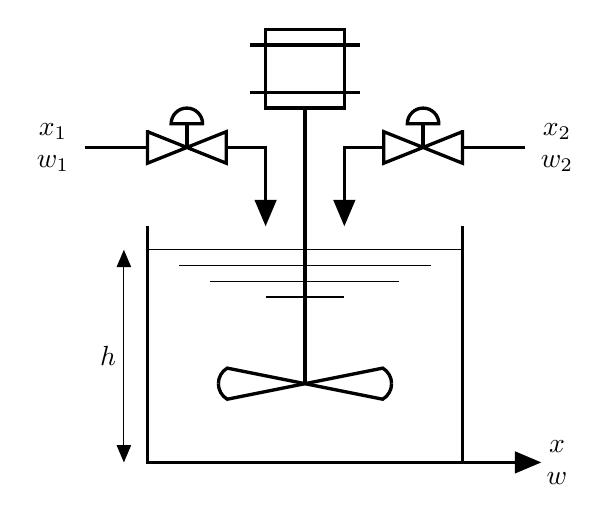
\begin{tikzpicture}[>=triangle 45]
%\draw[color=blue] (-2,-2) grid (11,11); %Tạo lưới
% Vẽ bình chứa
\drawe (0,3) -- (0,0) -- (4,0) -- (4,3);
\draw (0,2.7) -- (4,2.7);
\draw (0.4,2.5) -- (3.6, 2.5);
\draw (0.8,2.3) -- (3.2, 2.3);
\draw (1.5,2.1) -- (2.5, 2.1);
\drawe (-.8, 4) -- (0,4);
\drawe (0,4.2) -- (1,3.8) -- (1,4.2) -- (0,3.8) -- (0,4.22);
\drawe (0.5,4) -- (0.5, 4.3);
\drawe (0.7,4.3) arc (0:180:0.2) -- (0.72,4.3);
\drawe (1,4) -- (1.52,4);
\drawe[->] (1.5, 4) -- (1.5, 3);

\drawe (4.8, 4) -- (4,4);
\drawe (4,4.2) -- (3,3.8) -- (3,4.2) -- (4,3.8) -- (4,4.22);
\drawe (3.5,4) -- (3.5, 4.3);
\drawe (3.7,4.3) arc (0:180:0.2) -- (3.72,4.3);
\drawe (3,4) -- (2.48,4);
\drawe[->] (2.5, 4) -- (2.5, 3);

\draw (-1.2,4.2) node{$x_1$};
\draw (-1.2,3.8) node{$w_1$};

\draw (5.2,4.2) node{$x_2$};
\draw (5.2,3.8) node{$w_2$};

\draw[<->] (-0.3,0) -- (-0.3,2.7);
\draw (-0.5, 1.35) node {$h$};

% Vẽ máy khuấy trộn
\drawe (1.5,5.5) rectangle (2.5,4.5);

\drawe (1.3,5.3) -- (2.7,5.3);
\drawe (1.3,4.7) -- (2.7,4.7);
\drawe (2,4.5) -- (2, 1);
\drawe (1,0.8) -- (3,1.2);
\drawe (1,1.2) -- (3,0.8);
\drawe (3.1,1) arc (0:60:.23);
\drawe (3.1,1) arc (0:-60:.23);

\drawe (.9,1) arc (180:120:.23);
\drawe (.9,1) arc (180:240:.23);


% Vẽ ngõ ra
\drawe[->] (4,0) -- (5,0);
\draw (5.2,.2) node{$x$};
\draw (5.2,-.2) node{$w$};

\end{tikzpicture}
\end{document}